\documentclass[twocolumn,nofootinbib,showkeys,twoside,floatfix,unsortedaddress,flushbottom,10pt,aps,pra]{report}
\input  4mbapreamble
\usepackage{tikz}
\usepackage{latexsym}% 
\usepackage{graphics,graphicx}
\usepackage{amssymb}% 
\usepackage{amsmath}
\usepackage{amsfonts} % mathbb
\usepackage{natbib}% 
\usepackage{fancyhdr,lastpage}
\usepackage{titlesec}
\usepackage{bold-extra}
%\usepackage[margin=0.7in,headheight=60pt]{geometry}
\usepackage[width = 18cm, height = 22cm,headheight=70pt, columnsep = 1cm]{geometry}

\usepackage{lipsum}% http://ctan.org/pkg/lipsum
\usepackage{float}
\usepackage{listings}
\usepackage{subfigure}
\usetikzlibrary{shapes.geometric, arrows}
\tikzset{
  int/.style={circle, draw=black, fill=green!20, minimum size=3em},
  int1/.style={circle, draw=black, fill=red!20, minimum size=3em},
  int2/.style={circle, draw=black, fill=blue!20, minimum size=3em},
  init/.style={pin distance=1.2cm,pin edge={loop,thin,black}}
}
\tikzstyle{arrow} = [thick,black,->,>=stealth]
\tikzstyle{pinstyleto} = [pin edge={<-,thick,black}]
\tikzstyle{pinstyleout} = [pin edge={->,thick,black}]


\newcommand\numberthis{\addtocounter{equation}{1}\tag{\theequation}}
%\newcommand{\R}{{\cal R}}
%\newcommand{\Rlogo}{\protect
\includegraphics[height=2ex,keepaspectratio]{images/Rlogo.pdf}\xspace}

\AtBeginDocument{%
\renewcommand{\thesection}{\arabic{section}}%
\renewcommand{\contentsname}{\sc{\bfseries Contents}}
\renewcommand{\bibname}{\sc{\bfseries Bibilography}}
}

\author{\sc{\bfseries Model Students:}\\
\small \emph{Nicole Dumont \footnote{dumontns@mcmaster.ca}} \\
 \small \emph{Melody Fong \footnote{fongm5@mcmaster.ca}} \\
 \small  \emph{Carolina Weishaar \footnote{weishamc@mcmaster.ca}}}  
 \title{ \small \emph{Mathematics 4MB3/6MB3: Mathematical Biology }\\
  \Huge \sc{\bfseries Spatial Epidemics Dynamics:\\ Synchronization}}
  \date{\today \\
  Word Count: }
  

%\renewcommand{\abstractname}{\Huge \sc{Executive Summary}}

  \titleformat{\section}
  {\centering \normalfont \bfseries \scshape }{\thesection}{1em}{}
  
  \titleformat{\subsection}
  {\centering \normalfont \itshape \bfseries}{\thesubsection}{1em}{}



\lhead{\sc{Synchronization}}
\rhead{\emph{Model Students}} 
\renewcommand\headrulewidth{0pt}% Removes funny header line
\begin{document}



\pagestyle{fancy}

\maketitle
\tableofcontents

\onecolumn
\section*{\Huge Executive Summary}

The synchronicity of incidence data has been shown to inhibit rescue effects, thereby increasing the probability of eradicating disease \cite{McCluskey2011}. 

\addcontentsline{toc}{section}{\protect\numberline{}Executive Summary}%

The synchronicity of incidence data has been shown to inhibit rescue effects, thereby increasing the probability of eradicating disease \cite{McCluskley2014}. 



\twocolumn

\section{Abstract} Text goes here.
\section{Literature Review }
Long-term incidence records of many childhood diseases, such as measles, exhibit recurrent epidemics with  both regular (annual, biannual and even tri-annual cycles) and irregular dynamics \cite{Earn2000}. In countries where measles immunization is systematically distributed at 15 months and at 6 years, the observed amplitude of the incidence curve declines and the period of the epidemics become more irregular. However, overall this does not antagonize the natural dynamics of the disease \cite{Samanta2014,Earn2000}. As a result in order to increase the efficiency of control health care measures, it is essential to understand the factors that allow a follow up epidemic to occur after the aversion of an epidemic. In regards to childhood diseases, researchers have previously speculated that the phenomena of recurrence can be attributed to factors such as ***** (add citation and list parameters). However, many of these models have been found to be ineffective or possibly overfitted (citation). 
\par
\smallskip \qquad
One characteristic of disease spread that has been found to accurately induce persistence within compartmental models is spatial dynamics. To induce this property a metapopulation model is utilized, where the population is divided into several discrete subclasses, called patches, each exhibiting a well-mixed population. This model is analogous to the observed population distribution within countries, where the population is concentrated throughout towns and cities. As a result, subpopulations can exhibit a variety of states, which are out of phase in contrast to, the disease state observed by the entire population. For example, weekly incidence measles data from Birmingham, Newcastle, Cambridge and Norwich recorded between 1944 and 1958, clearly show that the epidemics are in phase in Birmingham and Newcastle and out of phase in Cambridge and Norwich \cite{Grenfell2001}. Asynchronous dynamics facilitate rescue effects, where the dispersal from patches with a large population prevents local extinctions in patches with small populations, thereby prolonging the eradication of disease. Hence, synchrony inhibits such processes, and could have a strong influence on the vulnerability of a disease from becoming eradicated globally. In addition to this, the facilitation of migration in modern society has allowed synchronicity to be of importance on a larger scale \cite{McCluskey2011}. For example in the case of Hepatitis B, Gay and Edmunds argue that it would be more cost effective for the United Kingdom to sponsor a vaccination program in Bangladesh than a national universal program \cite{Burton2012}. 
\par
\smallskip \qquad
In this study, we have used a metapopulation model where, the state of each patch is modelled by the susceptible, infectious and removed ($SIR$) model. The parameters chosen are based on the expected $R_0$ value for measles.  In addition to this, this study makes use of sinusoidal seasonal forcing on the transmission rate, in order to estimate the effects of vacation on the contact rate between the infectious and susceptible population, as opposed to the school year. The aim of this study is to analyze the dynamics of this model overtime, in order to determine which parameters lead to a synchronous state, thereby eradicating the disease. \par
\smallskip

\section{Methods}
\subsection{The Meta-patch SIR Model} 
\indent
The spatial SIR model consists of $n$ identical patches (which represent cities or some other spatial grouping of people) with identical population sizes. The population is constant in each patch and there is no migration between patches. Intra-patch dynamics are given by the standard SIR model with vital dynamics and sinusoidal seasonal forcing. Connectivity between patches is represented by disease transmission. Infected individuals can infect people from other patches. This models individuals visiting other patches, creating additional sources of infection in the visited patch. 
A visualization of the dynamics in a single patch $i$ is shown by
\begin{center}
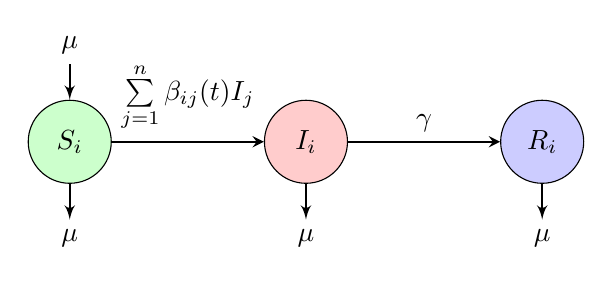
\begin{tikzpicture}[node distance=3cm,auto,>=latex',every node/.append style={align=center}]
    \node [int, pin={[pinstyleto]above:$\mu$}, pin={[pinstyleout]below:$\mu$}] (a)              {$S_i$};
    \node [int1, pin={[pinstyleout]below:$\mu$}] (b) [right of=a] {$I_i$};
    \node [int2, pin={[pinstyleout]below:$\mu$}] (c) [right of=b] {$R_i$};
    
    \draw [arrow] (a) -- node[anchor=south] {$ \sum\limits_{j=1}^{n}\beta_{ij}(t) I_j $} (b);
    \draw [arrow] (b) -- node[anchor=south] {$\gamma$} (c);
\end{tikzpicture}
\end{center}
\qquad
where $S_i$ is the proportion of the population in patch $i$ that is susceptible to becoming infected, $I_i$ is the proportion of the population that is infected, and $R_i$ is the proportion of the population that has recovered and now has lifelong immunity to the disease. $\frac{1}{\mu}$ is the average life expectancy, and $\frac{1}{\gamma}$ is the mean infectious period.
\par
 \smallskip \qquad
The equations describing the dynamics in a single patch are
\begin{align*}
  \frac{dS_i}{dt} &= \mu - S_i\sum\limits_{j=1}^{n}\beta_{ij}(t) I_j -\mu S_i \\ 
  \frac{dI_i}{dt} &= S_i\sum\limits_{j=1}^{n}\beta_{ij}(t) I_j -\gamma I_i - \mu I_i  \numberthis \label{model} \\
  \frac{dR_i}{dt} &= \gamma I_i -\mu R_i      
\end{align*}
where $S$ is the proportion of the population that is susceptible to infection, $I$ is the proportion of the population that is infectious, and $R$ is the proportion of the population that has recovered from the disease (and  have lifelong immunity) or who have died as a result of the disease. $\mu$ is the birth/death rate, $\gamma$ is the recovery rate, and $\beta_{ij}(t)$ are the elements of the $n\times n$ matrix $\beta(t)$:
\begin{equation}
  \beta(t) = \left < \beta \right > (1+\alpha \cos(2\pi t))M
\end{equation}
$\left < \beta \right > (1+\alpha \cos(2\pi t))$ is the standard sinusoidal forced transmission rate. $M$ is a matrix describing the connectivity between patches. Its $(i,j)$ element is the proportion of contacts of individuals in patch $i$ make with individuals in patch $j$. The off-diagonal elements are generally less than the diagonal elements since it is usually assumed individuals have more contact with people in their own patch. $M$ is assumed here to be symmetric - i.e. patch $i$ has as much contact with patch $j$ as $j$ does with $i$. The column sums of $M$ (and thus the rows sums too) are all equal to one - i.e. $M$ is doubly stochastic. This means that all of an individual's time is accounted for. 
\par \smallskip \qquad
Two different types of $M$ matrices are used in this paper. The first is equal coupling where all patches are equally connected, i.e. all off-diagonal elements of $M$ are equal. The fraction of time individuals spend outside their own patch is given by the parameter $m$.
\[
M =
\begin{bmatrix}
  1-m & \frac{m}{n-1} & \frac{m}{n-1} & \frac{m}{n-1} \\
  \frac{m}{n-1} & 1-m & \frac{m}{n-1} & \frac{m}{n-1}  \\
  \frac{m}{n-1} & \frac{m}{n-1} & 1-m &  \\
  \frac{m}{n-1} &  &  & \ddots 
\end{bmatrix}
\]
The second motif is nearest neighbour coupling. In this case it is assumed that the patches reside on a ring and people can only visit their two nearest neighbours.
\[
M =
\begin{bmatrix}
  1-m & \frac{m}{2} & 0 & 0 & \dots & \frac{m}{2} \\
  \frac{m}{2} & 1-m & \frac{m}{2} & 0 & & \vdots \\
  0 & \frac{m}{2} & 1-m &  \\
  0 & 0 & & \ddots \\
  \vdots & & & & \ddots & \frac{m}{2} \\
  \frac{m}{2} &  & & \dots & \frac{m}{2} & 1-m \ 
\end{bmatrix}
\]
Realistic connectivity probably lies between these two extreme motifs \cite{Earn2000}.\par
 \smallskip \qquad
 A solution to this model is said to be coherent if at all times, $I_1(t)=I_2(t)=...=I_n(t)$ for all $n$ patches \cite{McCluskey2011} - i.e. all states are equal to the mean $I_i(t)=\left < I(t) \right > $. A solution is less coherent the further all states are from the mean. We use the coefficient of variation (also called the relative standard deviation) as a measure of how coherent a solution is. The coefficient of variation is the standard derivation of the set $\{I_i(t)\}_{i=1}^n$ divided by the mean of the set. If it is zero for all time, the solution is coherent.

\section{Results}
\subsection{Periods of Single Patch Model }
\indent
A bifurcation diagram was created using \verb|XPPAUT|.
This produces a bifurcation diagram which shows the periodic recurrence patterns for the simulated deterministic model of the epidemic pattern. As shown in Figure \ref{fig:bifurcation}, there is a single period 1 orbit for $\{5<\R_0\}\cap\{\R_0>27\}$ as well as a single period 2 orbit for $15<\R_0<25$ and mixed dynamics elsewhere.
\begin{figure}[H]
    \caption{A bifurcation diagram for the single patch sinusoidal forced SIR model.}
    \label{fig:bifurcation}
    \centering
    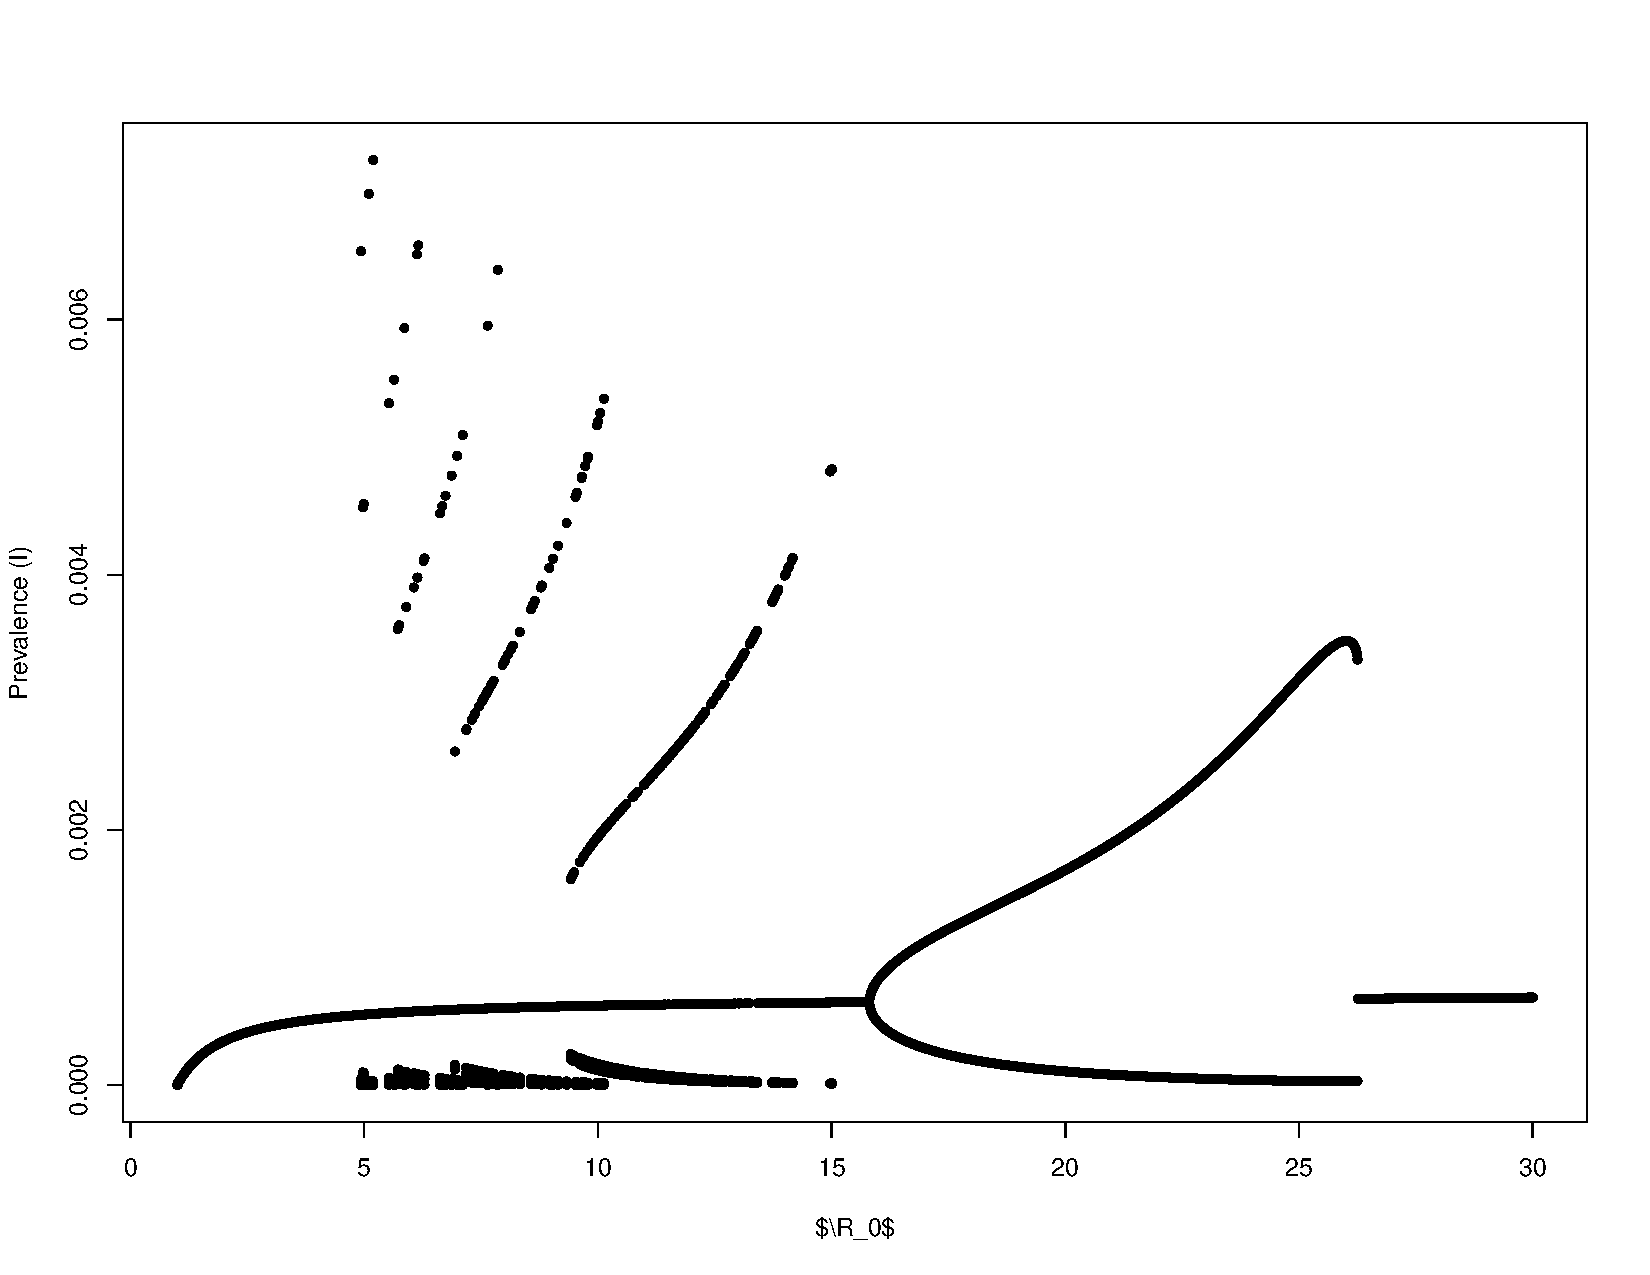
\includegraphics[width=\linewidth]{{images/bifurcation}.pdf}
\end{figure}
Further analysis of the bifurcation diagram reveal the period compositional structure. See Figure \ref{fig:period}.
\begin{figure}[H]
    \caption{The periods of the single patch sinusoidal forced SIR model vs parameter $\R_0$.}
    \label{fig:period}
    \centering
    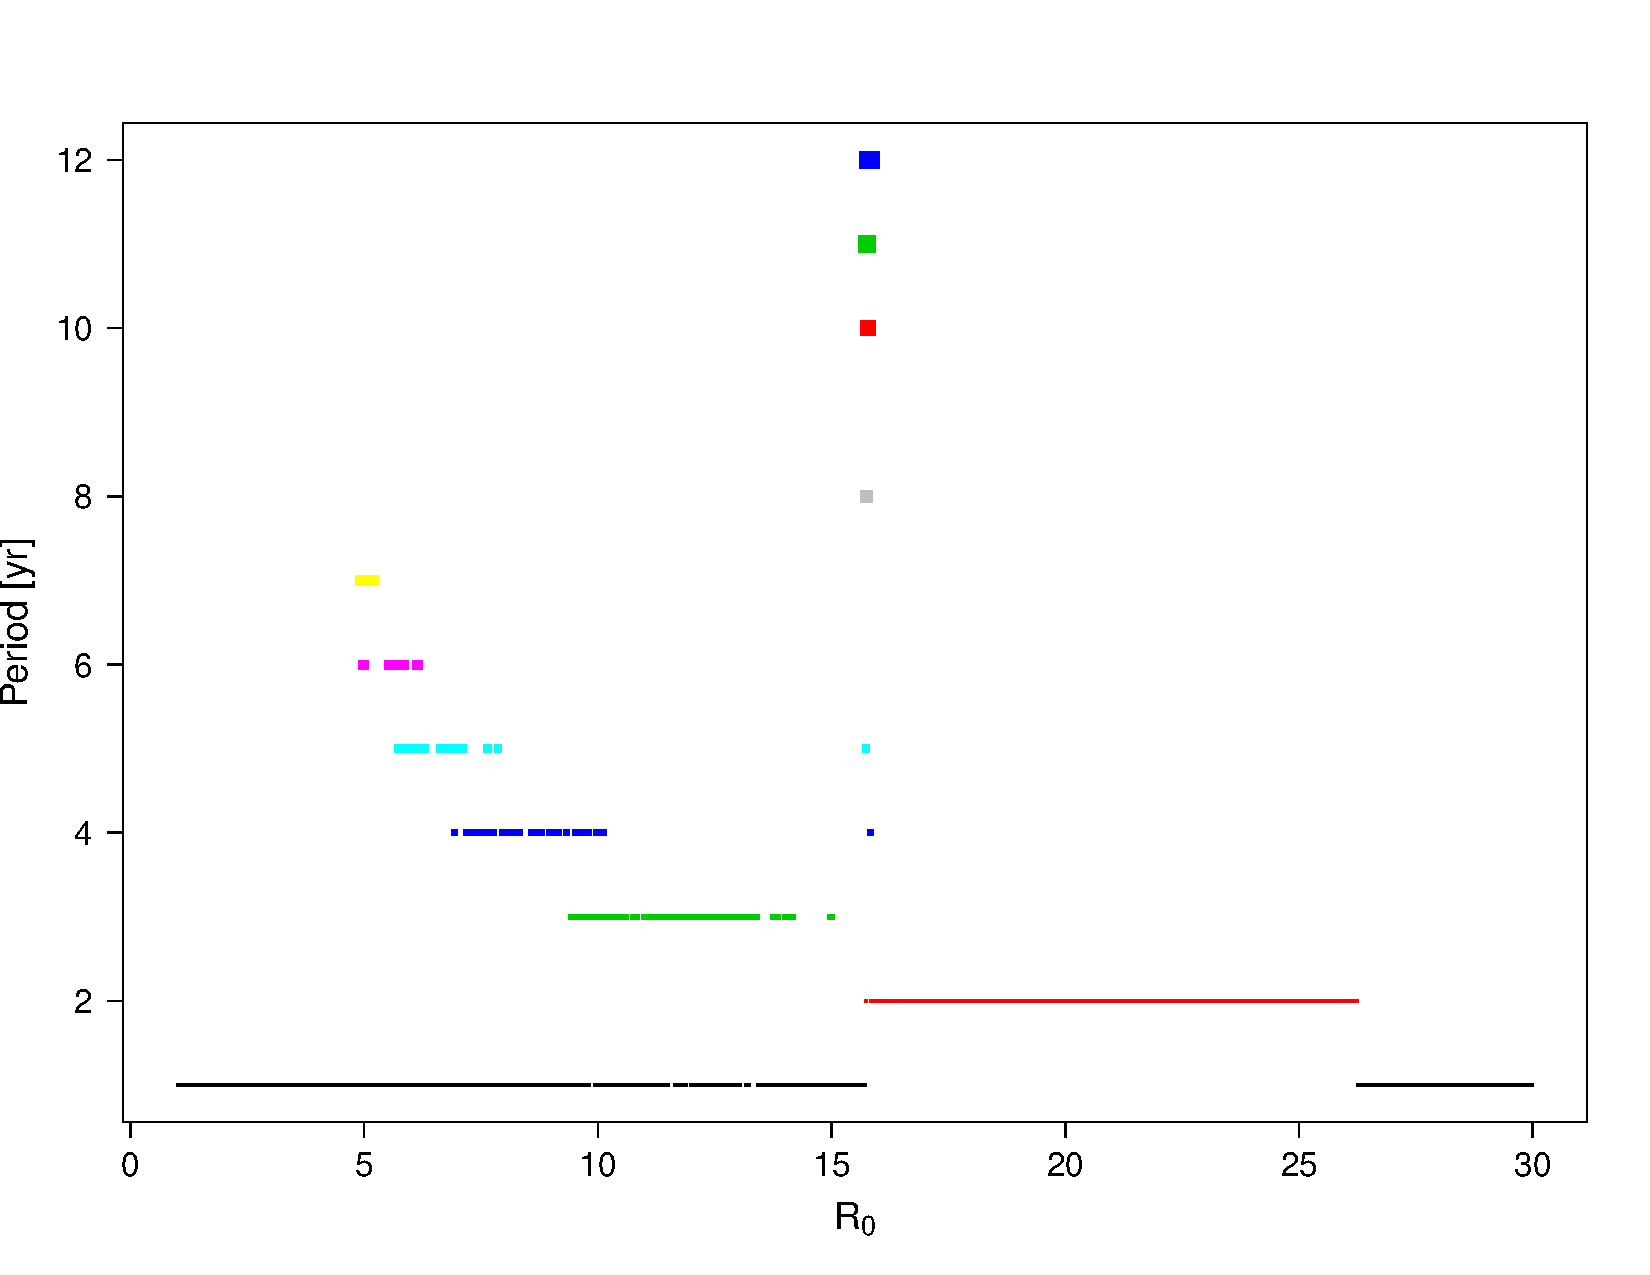
\includegraphics[width=\linewidth]{{images/period}.pdf}
\end{figure}


\begin{figure*}
    \caption{$\R_0=17$ and $m=0.2$}
    \label{fig:detplotsC}
    \centering
    \subfigure[Equal Coupling]
    {
        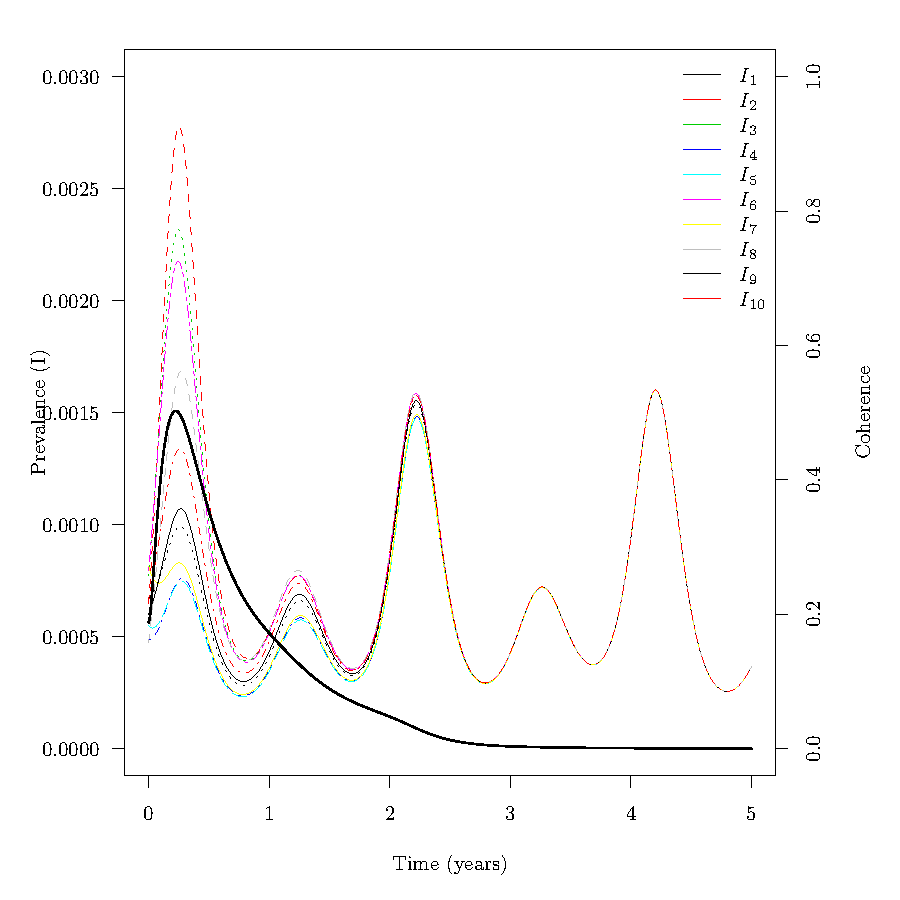
\includegraphics[width=3.0in]{{images/detECR017m0.2s}.pdf}
    }
    \subfigure[Nearest Neighbour Coupling]
    {
        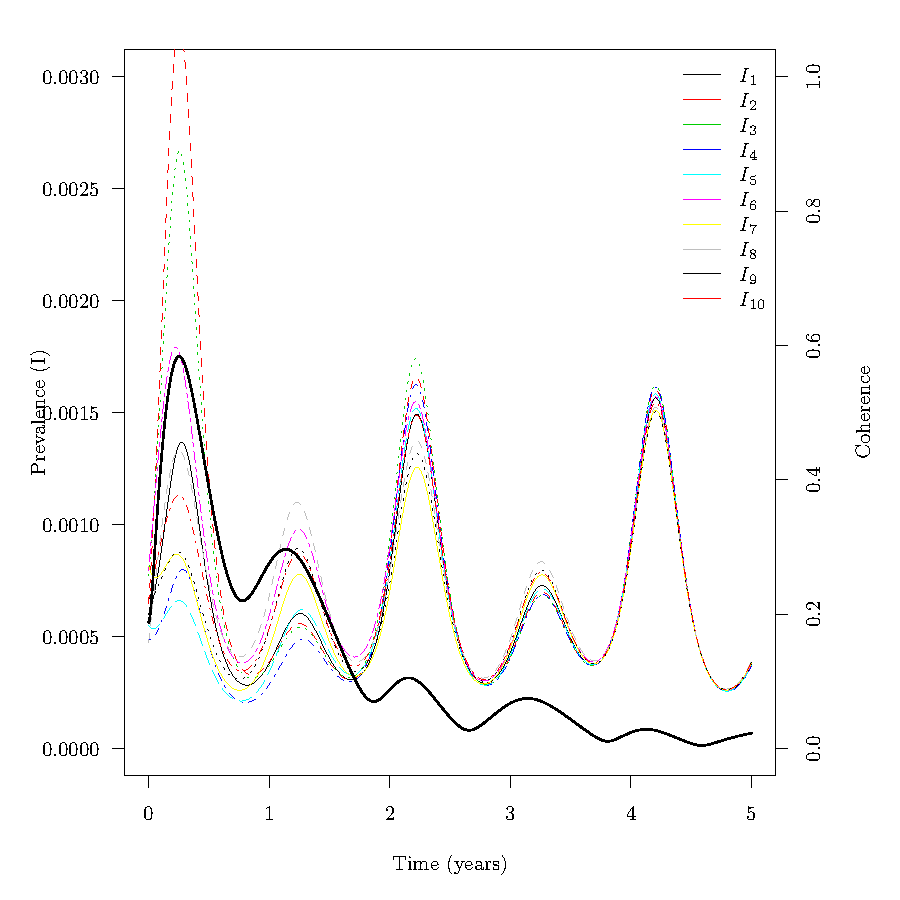
\includegraphics[width=3.0in]{{images/detNNR017m0.2s}.pdf}
    }
\end{figure*}
\begin{figure*}
    \caption{Nearest Neighbour Coupling, $m=0.2$}
    \label{fig:detplotsR0}
    \centering
    \subfigure[$\R_0=10$]
    {
        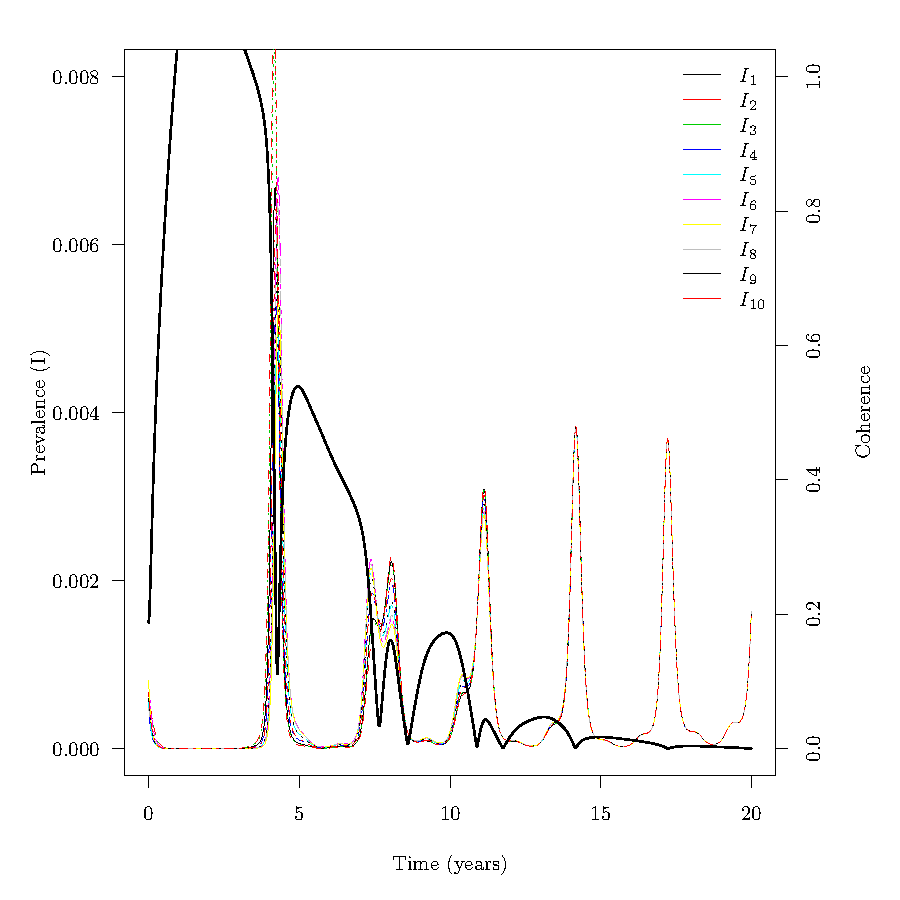
\includegraphics[width=3.0in]{{images/detNNR010m0.2}.pdf}
    }
    \subfigure[$\R_0=25$]
    {
        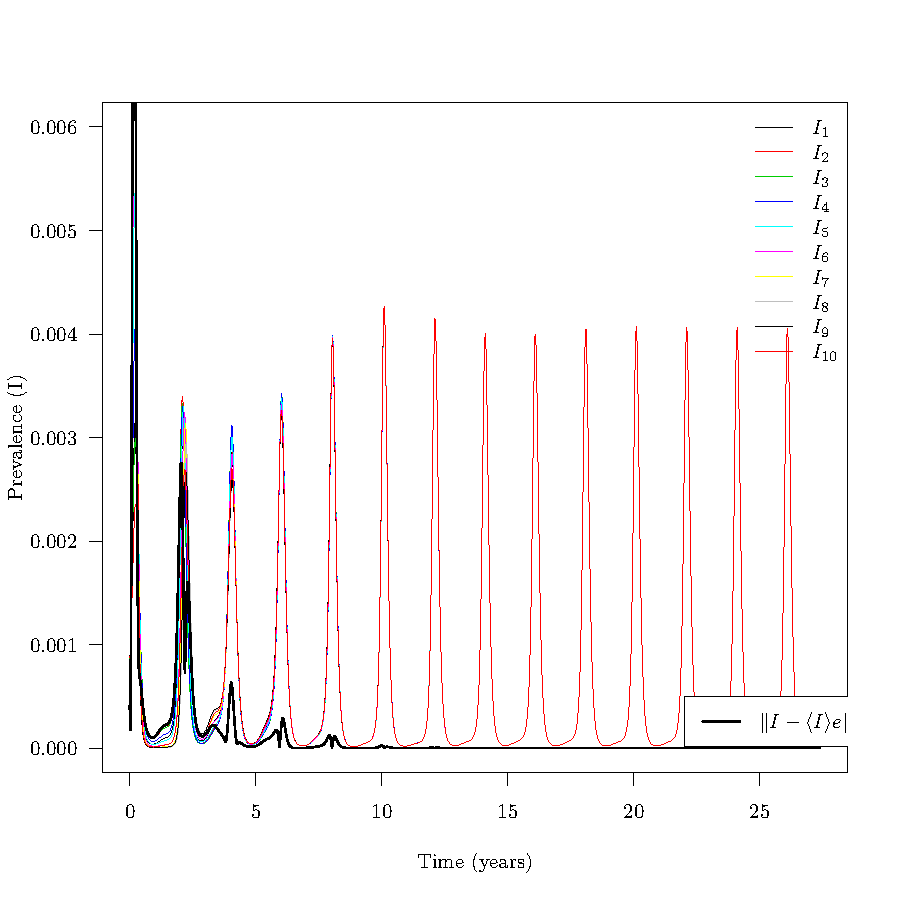
\includegraphics[width=3.0in]{{images/detNNR025m0.2}.pdf}
    }
\end{figure*}
\begin{figure*}
    \caption{Nearest Neighbour Coupling, $\mathcal{R}_0=17$, $m=0.01$}
    \label{fig:detplotsm}
    \centering
    \subfigure[Within 30\% percent of endemic equilibrium]
    {
        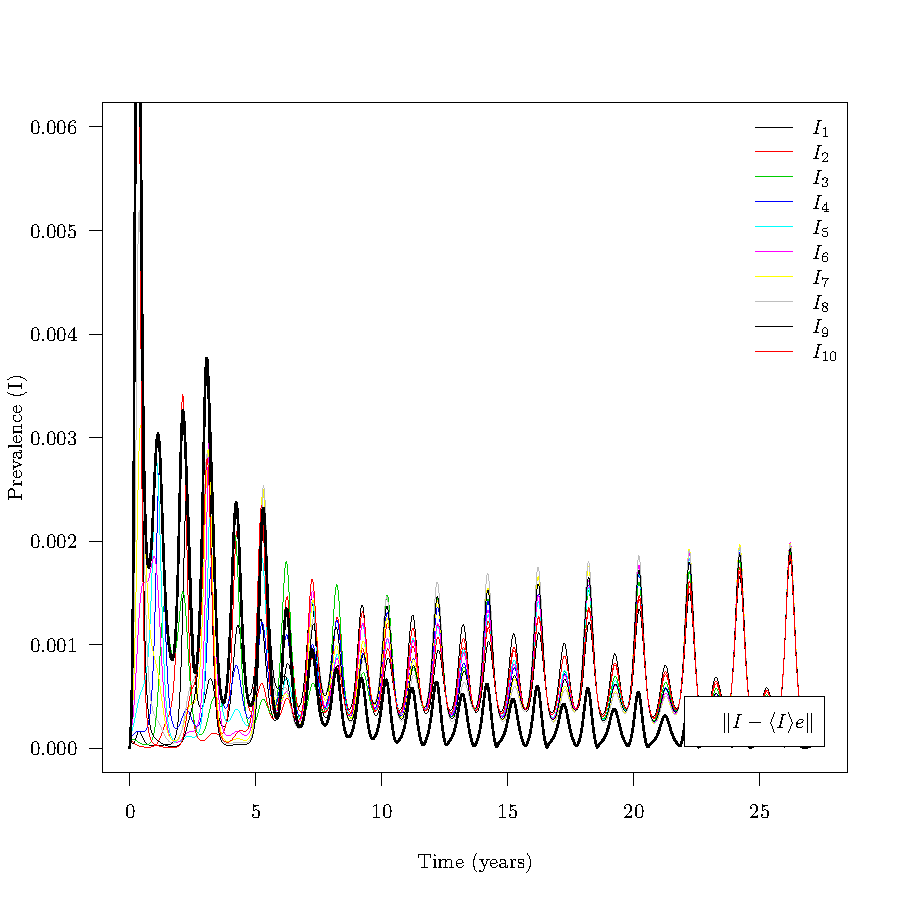
\includegraphics[width=3.0in]{{images/detNNR017m0.01}.pdf}
    }
    \subfigure[Within 40\% percent of endemic equilibrium]
    {
        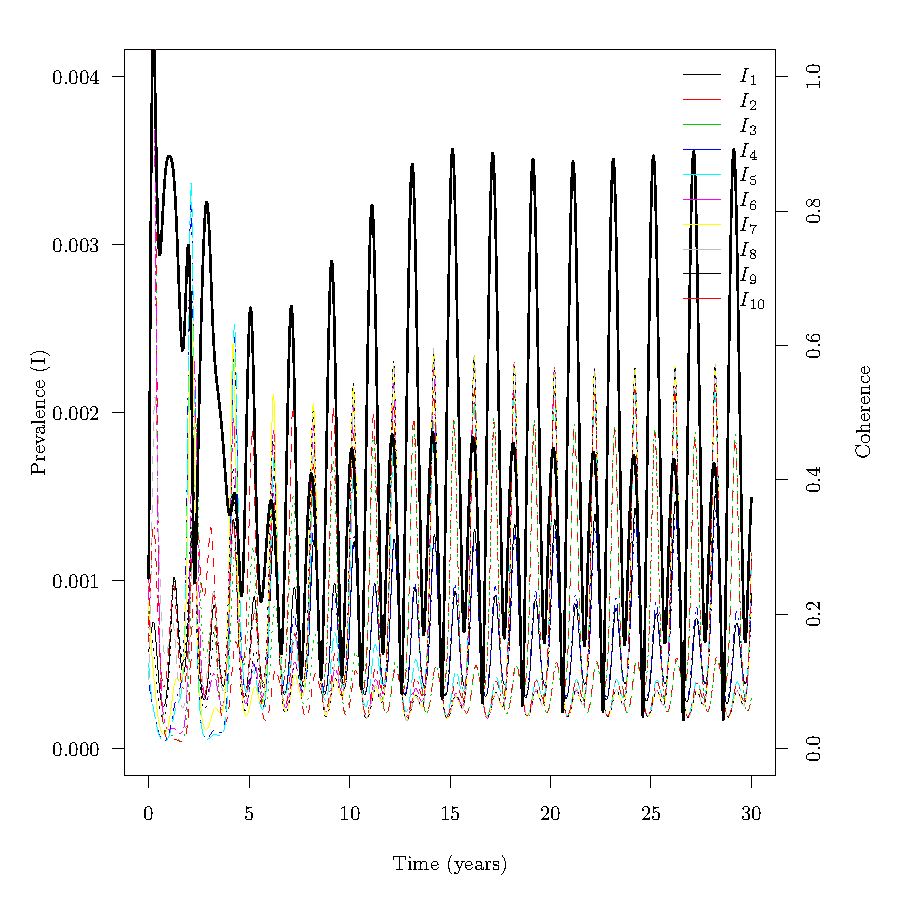
\includegraphics[width=3.0in]{{images/detNNR017m0.01wider}.pdf}
    }
    \end{figure*}

\subsection{Deterministic Solution}
Solutions to \eqref{model} were calculated using the \Rlogo \texttt{deSolve} package. 
The following figures are the solutions for a 10 patch model with a 50 year life expectancy, a 13 day mean infectious period, and seasonal forcing amplitude $\alpha = 0.1$. The initial conditions used were values within $\pm30\%$ of the $(S,I,R)$ values at the Endemic Equilibrium of the unforced single patch SIR model. In Figure \ref{fig:detplotsC} values of $\R_0=17$ and $m=0.2$ were used and the difference between equal coupling and nearest neighbour coupling is shown. It takes longer for solutions to become coherent when using nearest neighbour coupling. \par
 \smallskip \qquad

Figure \ref{fig:detplotsR0} shows the different oscillatory periods of the epidemic cycles for two different values of $\R_0$. 
In Figure \ref{fig:detplotsm} weaker connectivity was used, $m=0.01$.  Solutions became coherent even at this low $m$ if the initial conditions are close enough to the Endemic Equilibrium values. 

\subsection{Stochastic Simulations} 
\indent
A stochastic version of this model was simulated approximately using the adaptive tau-leaping algorithm. The same parameters and similar initial conditions to the ones used for the deterministic solution were used. Figure \ref{fig:adapplot} shows two stochastic simulations with $\R_0=17$ and a population of 500,000.

\begin{figure*}
    \caption{An approximate stochastic simulation using the adaptive tau-leaping method.}
    \label{fig:adapplot}
    \centering
    \subfigure[$m=0.2$]
    {
        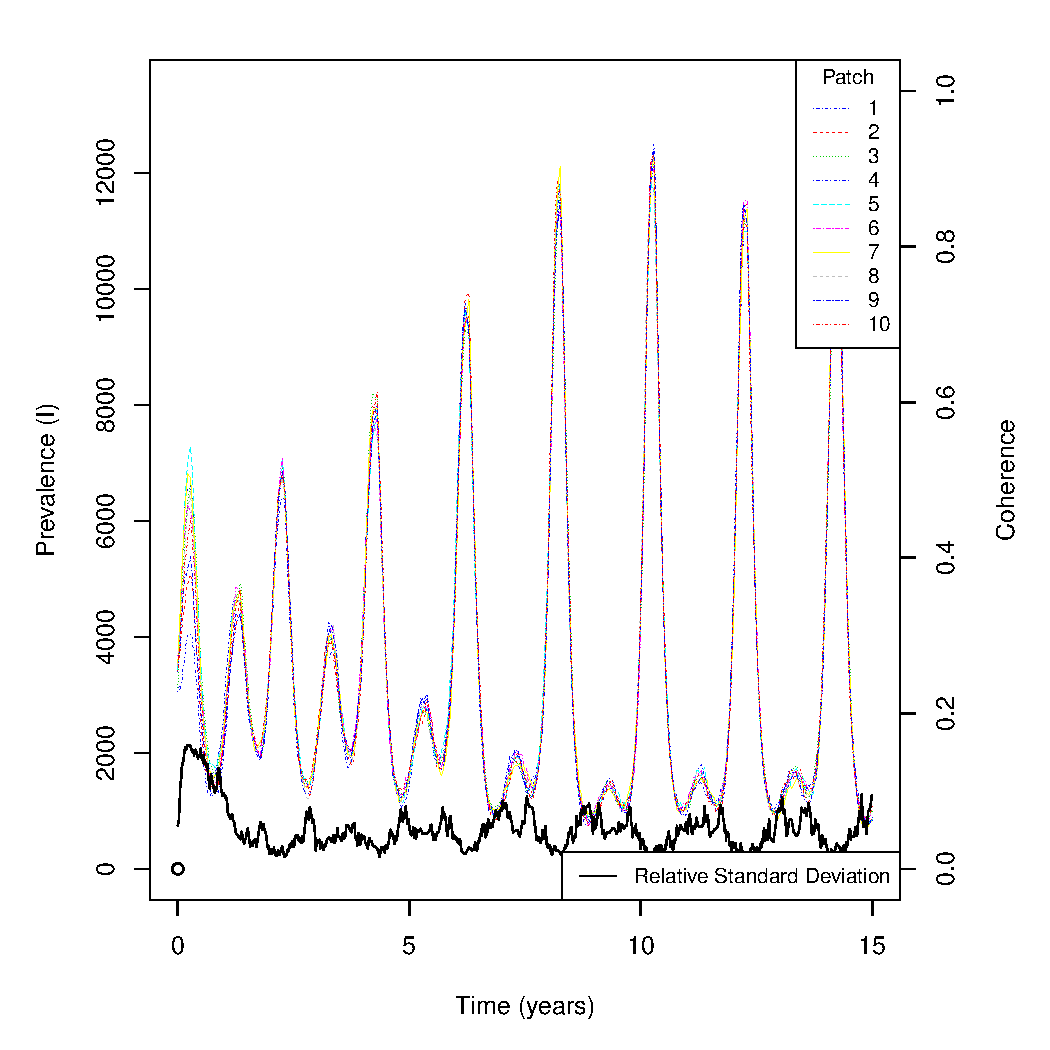
\includegraphics[width=3.0in]{{images/adaptauECR017m0.2}.pdf}
    }
    \subfigure[$m=0.01$]
    {
        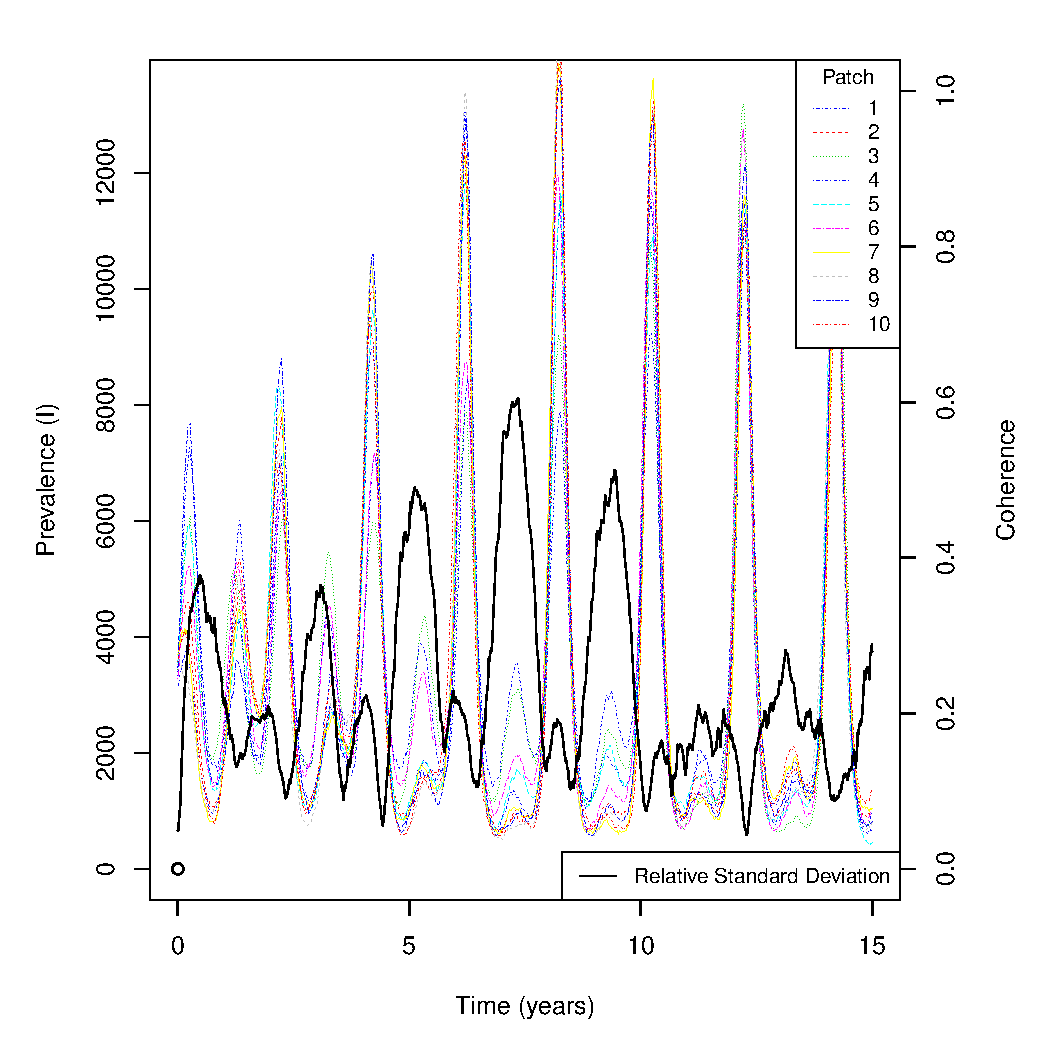
\includegraphics[width=3.0in]{{images/adaptauECR017m0.01}.pdf}
    }   
\end{figure*}

\subsection{Coherence Dependence Parameters} 
The affect parameters had on coherence was investigated. A $100\times100$ grid of $\R_0$ and $m$ values was created. At each grid point an approximate stochastic simulation was run ten times each with different initial conditions (all within $10\%$ of the Endemic Equilibrium values) and the measure of coherence during the $9^{th}$ year of the simulation was recorded. If the measure of coherence was below a threshold value of $0.15$ (i.e. the states were within $15\%$ of the mean value), the simulation was said to be coherent. From this the probability of a solution becoming coherent for different $\R_0$ and $m$ was determined. See Figure \ref{fig:3D}. \par
 \smallskip \qquad Figure \ref{fig:4pan} shows the probability of local extinction (the probability that the infected population of any given individual patch will go below a small threshold value), the probability of global extinction (the probability that the infected population of all patches will go below a small threshold value) in addition to the probability of coherence for different parameters\par
 \smallskip \qquad
 Both of these figures are reproductions of Figs. 2 and 3 in \citet{Earn2000} using the forced meta-patch SIR model in lieu of the logistic map function. 
\begin{figure*} 
    \caption{3D plots of the probability of coherence at $\R_0$ values between 2 and 30, and $m$ values between 0 and 0.9.}
    \label{fig:3D}
    \centering
    \subfigure[Nearest Neighbour Coupling]
    {
        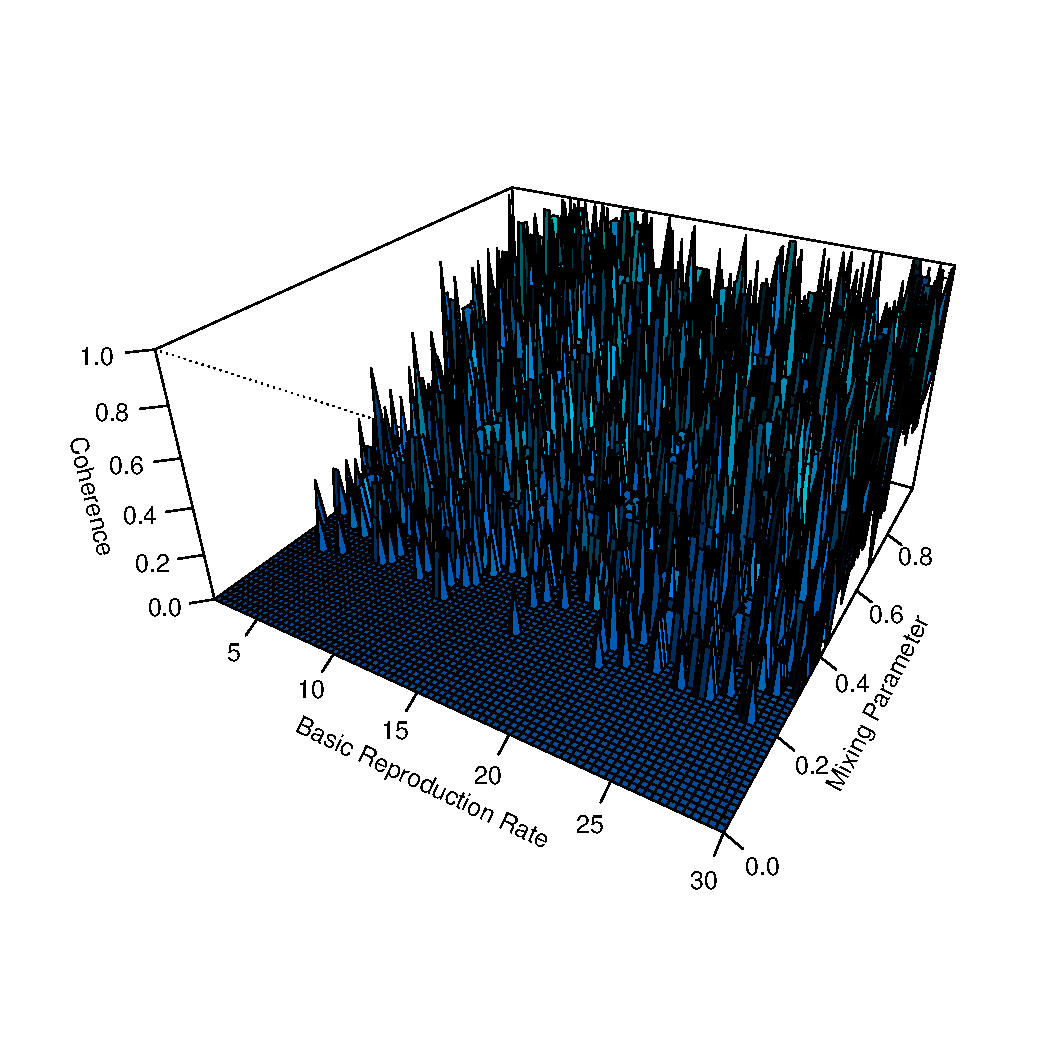
\includegraphics[width=3.0in]{{images/Adaptau3DNN}.pdf}
    }
    \subfigure[Equal Coupling]
    {
        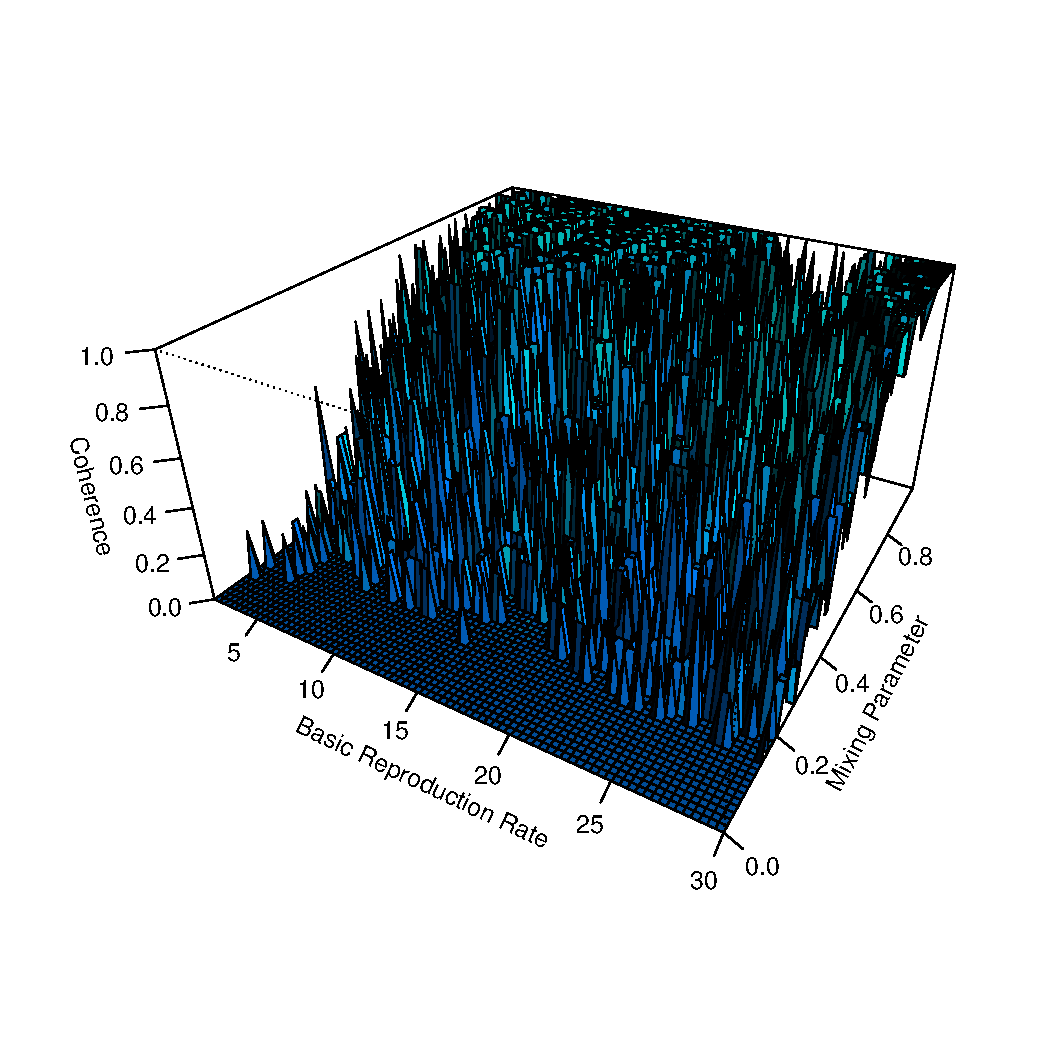
\includegraphics[width=3.0in]{{images/Adaptau3DEC}.pdf}
    }   
\end{figure*}

\begin{figure*}
    \caption{The probability of coherence, local extinction, and global extinction at $\R_0$ values between 2 and 30 for four different $m$ values. Below each plot is the bifurcation diagram of the single patch model.}
    \label{fig:4pan}
    \centering
    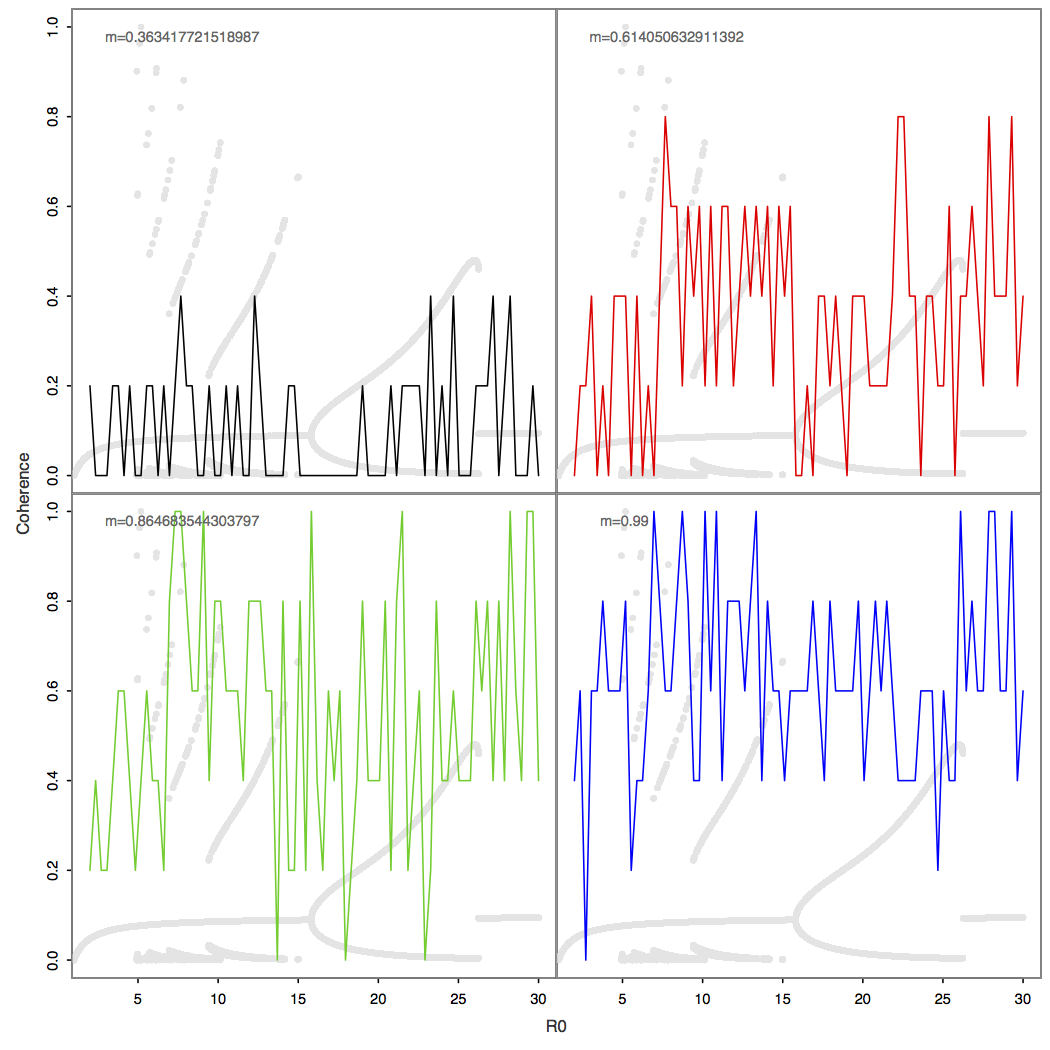
\includegraphics[width=\linewidth]{{images/FourPanelNN}.pdf}
\end{figure*}

\section{Discussion} 
\textit{(i) First two figs $<-$ there exist local convergence around 30$\%$ of the endemic equilibrium (where there is asymptotic stability for $\R_0 > 1$), so results so stick within that region \textbf{[Note: maybe mention this in results somewhere (included in v2 of supplementary)]}
(iii) Third two figs $<-$ relation between $\R_0$ and coherence \textbf{[Note: not much info here - can remove or change to show more varied dynamics between two $\R_0$ parameters]}]}
\bigskip
The most evident parameter affecting the synchronization of the multipatch system is the connectivity. As shown in \ref{fig:adapplot}, for two models under the same connectivity relation (equal coupling), the one with higher mixing parameter $m$ is more likely to become coherent for all time. This relationship is shown on a larger scale in Fig. \ref{fig:3D} with the general trend of the surface sloping towards total coherence for increasing mixing parameter $m$. In general, this result indicates that, for example, when only changing the system by restricting the mixing of the disease by around $20\%$, coherence decreases from $95.2\%\pm2.43\%$ to $77.3\%\pm12.5\%$ \textbf{[Note: Axis of coherence adapplot change from 1-0]}. Therefore, in theory, increasing contact between population patches would greatly aid in synchronizing the system. However, while a synchronized system is predicted to reduce the likelihood of the "rescue effect" \cite{Earn2000}, it should be noted that other parameters such as the number of secondary infections, $\R_0$, would be affected by any change in $m$. Consequently, further study on the effect of changing the mixing parameter in a system should be conducted prior to employing this result as a viable option to controlling epidemics. \par \smallskip \qquad
The system under equal coupling and nearest neighbour coupling exhibit similar dynamics, as shown in Fig. \ref{fig:detplotsC}, with convergence to a coherent solution occurring much slower for the nearest neighbour system. This relationship is expected as already established, coherence increases with the degree of mixing. Since the system under nearest neighbour coupling models less interpatch mixing overall, in comparison with equal coupling, for both models under identical conditions, the one with nearest neighbour coupling should coverge slower than the one with equal coupling. Alternate connectivity relations can be investigated to validate that this property has no effect on the overall convergence of the system to coherence, only the time scale in which the result can be predicted to occur. \par \smallskip \qquad
Through Fig. \ref{fig:3D}, there appears to be a relation between the basic reproduction number \textbf{[Note: If possible, change axis name to "Number" en lieu of "Rate" - presentation]} and coherence, with the surface appearing to display concavities at certain regions of $\R_0$. This relationship is further explored in Fig. \ref{fig:4pan} where, for high mixing, coherence is clearly seen to dip in regions corresponding to periods of less complex dynamics, especially in the period of bi-annual cycles between $15<\R_0<25$. But, this pattern of dipping is not seen in the period of annual cycles between $\{5<\R_0\}\cap\{\R_0>27\}$. Therefore, as stated in Earn, Levin, and Rohani, the results indicate that there is only a weak, if any, relation between chaos and population persistence\cite{Earn2000} and therefore, that of the parameter $\R_0$ and coherence. \par \smallskip \qquad
Instead, more consideration should be directed toward the deviations between local and global extinction in relation to probability of coherence. Deviations are lower for high mixing parameter and dips in global extinction rate in comparison to local extinction rate correspond closely to dips in coherence \textbf{[Note: May be too similar to what is stated in Earn2000 - pg.2 col.3 p.2 l.1]}. In context, this result implies that, for low coherence, the probability of global extinction is also relatively low. This is due to the fact that, while the probability of local extinction is relatively higher, coherence is low, so mixing from other patches at possibly higher rates of infecteds can lead to a rekindling of the disease in patches where local extinction occurred, that is, the "rescue effect" causing global extinction to stay proportionally low.
\section{Conclusion} 


\onecolumn
\addcontentsline{toc}{section}{\protect\numberline{}Bibilography}%
\bibliographystyle{vancouver}
\bibliography{ModelStudents} 
\end{document}
